L'idée est toute simple à comprendre. On commence en partant de la configuration gagnante pour trouver toutes les nouvelles configurations obtenues en faisant un seul mouvement.
À partir de ces nouvelles configurations, on en recherche d'autres nouvelles obtenues en faisant un second mouvement. Ceci peut se résumer par l'arbre ci-dessous où une configuration $\mathcal{C}_1$ est reliée à une autre $\mathcal{C}_2$ uniquement si l'on peut passer de $\mathcal{C}_1$ à $\mathcal{C}_2$ en un seul mouvement, et quand on descend dans l'arbre on ne garde que les nouvelles configurations.


\begin{center}
    \begin{tikzpicture}[
    rotate=0,
    level distance=1.5cm,
        level 1/.style={sibling distance=5cm},
        level 2/.style={sibling distance=2.25cm},
    ]
    \node{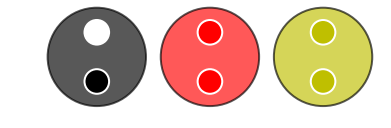
\includegraphics[scale=0.14]{content/optimal/tree_sol/moves/0.png}}
child{node{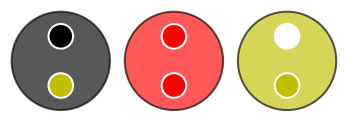
\includegraphics[scale=0.14]{content/optimal/tree_sol/moves/1.png}}
child{node{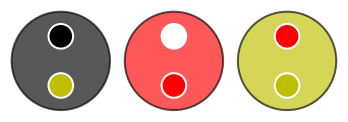
\includegraphics[scale=0.14]{content/optimal/tree_sol/moves/3.png}}}
child{node{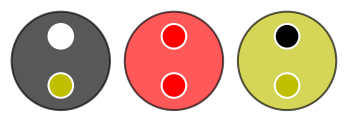
\includegraphics[scale=0.14]{content/optimal/tree_sol/moves/4.png}}}}
child{node{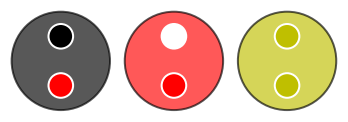
\includegraphics[scale=0.14]{content/optimal/tree_sol/moves/2.png}}
child{node{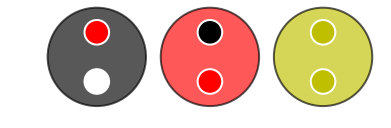
\includegraphics[scale=0.14]{content/optimal/tree_sol/moves/5.png}}}
child{node{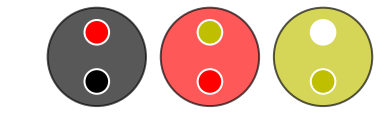
\includegraphics[scale=0.14]{content/optimal/tree_sol/moves/6.png}}}};
    \end{tikzpicture}
\end{center}



Avec un mouvement de plus, nous avons l'arbre ci-dessous qui à gauche perd sa symétrie.


\begin{center}
    \begin{tikzpicture}[
    rotate=0,
    level distance=1.5cm,
        level 1/.style={sibling distance=8.5cm},
        level 2/.style={sibling distance=4.75cm},
        level 3/.style={sibling distance=2cm},
    ]
    \node{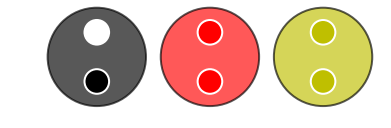
\includegraphics[scale=0.12]{content/optimal/tree_sol/moves/0.png}}
child{node{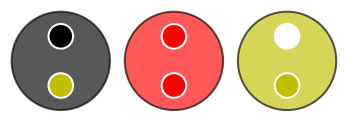
\includegraphics[scale=0.12]{content/optimal/tree_sol/moves/1.png}}
child{node{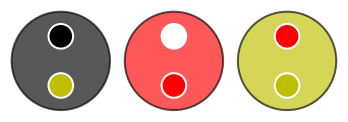
\includegraphics[scale=0.12]{content/optimal/tree_sol/moves/3.png}}
child{node{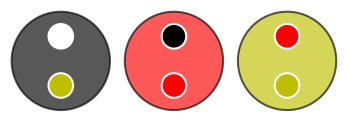
\includegraphics[scale=0.12]{content/optimal/tree_sol/moves/7.png}}}
child{node{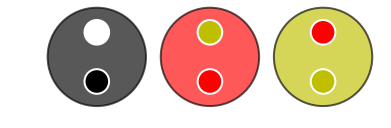
\includegraphics[scale=0.12]{content/optimal/tree_sol/moves/8.png}}}
child{node{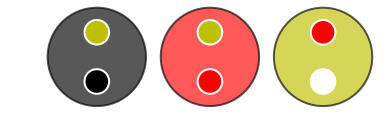
\includegraphics[scale=0.12]{content/optimal/tree_sol/moves/9.png}}}}
child{node{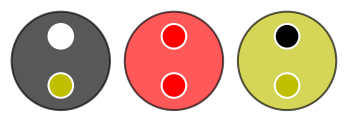
\includegraphics[scale=0.12]{content/optimal/tree_sol/moves/4.png}}
child{node{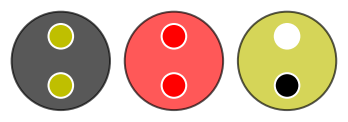
\includegraphics[scale=0.12]{content/optimal/tree_sol/moves/10.png}}}
child{node{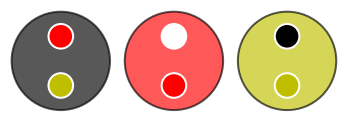
\includegraphics[scale=0.12]{content/optimal/tree_sol/moves/11.png}}}}}
child{node{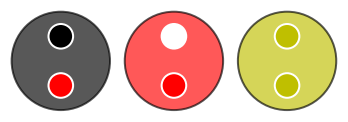
\includegraphics[scale=0.12]{content/optimal/tree_sol/moves/2.png}}
child{node{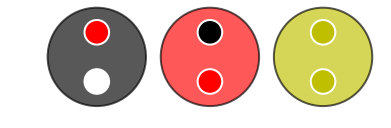
\includegraphics[scale=0.12]{content/optimal/tree_sol/moves/5.png}}
child{node{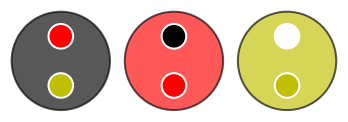
\includegraphics[scale=0.12]{content/optimal/tree_sol/moves/12.png}}}
child{node{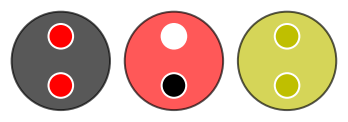
\includegraphics[scale=0.12]{content/optimal/tree_sol/moves/13.png}}}}
child{node{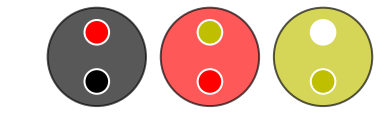
\includegraphics[scale=0.12]{content/optimal/tree_sol/moves/6.png}}
child{node{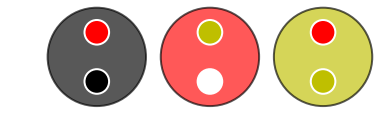
\includegraphics[scale=0.12]{content/optimal/tree_sol/moves/14.png}}}
child{node{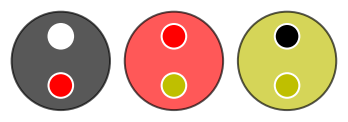
\includegraphics[scale=0.12]{content/optimal/tree_sol/moves/15.png}}}}};
    \end{tikzpicture}
\end{center}



Avec de la patience, ou grâce à un programme, on peut fabriquer l'arbre complet. Vous le trouverez en annexe. Notons que pour un jeu à cinq bases, il y a tout de même $11\,010$ configurations comme ceci est justifié dans l'annexe. Donc représenter l'arbre complet pour 5 bases sur une feuille A4, même avec l'aide d'un programme, ne sera pas possible. 


\medskip

????

idée que l'on en peut pas faire mieux, et traductiona lgorithmqiue, qui est un préalable pour programmer cette méthod qui n'est pas utilisable par humain (sauf à utiliser une armée de servants)


Voici l'algorithme qui va nous donner le moins possible de déplacements pour arriver à la configuration gagnante. Nous allons utiliser des dictionnaires qui sont des objets associant une valeur à une clé. Par exemple, $mon\_dico = \{"un": 1, "deux":2 \}$ admet pour clés $"un"$ et $"deux"$, et nous notons $mon\_dico\left["un"\right] = 1$ la valeur associée à la clé $"un"$.

\bigskip

\begin{algo}
	\Data{?????  une configuration quelconque de début de jeu}
	\Result{la solution gagnante en utilisant le moins possible de déplacements}
	\vspace{0.4em}
    \Begin{
		\vspace{0.4em}
		\tcp{Construction de toutes les configurations tout en gardant en mémoire le moins possible}
		\tcp{de déplacements pour accéder à chaque nouvelle  configuration construite.}
		???
		\\
		\vspace{0.4em}
		$\cal G$ désigne la configuration gagnante.
		\\
		\vspace{0.4em}
		\While{la configuration contient un jeton qui n'est pas dans sa base}{
			\vspace{0.4em}
			???
		}
		\vspace{0.4em}
		\tcp{????}
    }
\end{algo}


\bigskip

Les instructions étant sans ambiguïté, nous allons pouvoir nous attaquer très sérieusement à la validation des propriétés de \quote{finitude} et de \quote{résolution}.

\begin{proof}
	????????????????????
\end{proof}


\paragraph{Remarque :} ????
